\documentclass[aspectratio=169, pdf, 8pt, unicode]{beamer}
\usepackage[american,russian]{babel}
\usepackage[default]{sourcesanspro}
\usepackage{float}
\usepackage{graphicx}
\usepackage{pgfplotstable}
\usepackage{caption}
\usepackage{amsmath}
\usepackage{amssymb}
\usepackage{setspace}
\usepackage{fancyvrb}
\usepackage[outputdir=aux]{minted}

\DeclareCaptionLabelFormat{gostfigure}{Рисунок #2}
\captionsetup[table]{labelsep=endash,justification=justified,singlelinecheck=false,font=normalsize,skip=0pt} 
\captionsetup[figure]{labelformat=gostfigure,labelsep=endash,justification=centering,singlelinecheck=false,font=normalsize} 
\pgfplotsset{compat=1.9}

\mode<presentation> {
\usetheme{Madrid}
}

\setbeamerfont{institute}{size=\normalsize}
\setbeamertemplate{itemize/enumerate body begin}{\large}
\setbeamertemplate{itemize/enumerate subbody begin}{\tiny}

\title[Теория и практика многопоточного программирования]{Теория и практика многопоточного программирования\\ \vspace{0.5cm}Семинар 5}

\author{Неганов Алексей}

\institute[МФТИ]{
    Московский физико-технический институт (национальный исследовательский университет)\\
    Кафедра теоретической и прикладной информатики\\
}

\date{Москва 2020}

\setbeamertemplate{caption}[numbered]

\begin{document}

\begin{frame}
\titlepage
\end{frame}

\begin{frame}[fragile]
\frametitle{Spinlock}
\begin{figure}[H]
\centering
\begin{minipage}{0.8\textwidth}
\begin{minted}{C++}
class spin_lock_TAS
{
    atomic<unsigned int> m_spin ;
public:
    spin_lock_TAS(): m_spin(0) {}
    ~spin_lock_TAS() { assert( m_spin.load() == 0);}

    void lock() {
        unsigned int expected;
        do { expected = 0; }
        while ( !m_spin.compare_exchange_weak(expected, 1));
    }

    void unlock() {
        m_spin.store(0);
    }
};
\end{minted}
\end{minipage}
\end{figure}
\begin{block}{Вопрос}
Как в атомарных операциях расставить \texttt{memory\_order}?
\end{block}
\end{frame}

\begin{frame}[fragile]
\frametitle{Spinlock}
\begin{figure}[H]
\centering
\begin{minipage}{0.8\textwidth}
\begin{minted}{C++}
class spin_lock_TTAS
{
    atomic<unsigned int> m_spin ;
public:
    spin_lock_TTAS(): m_spin(0) {}
    ~spin_lock_TTAS() { assert( m_spin.load() == 0);}

    void lock() {
        unsigned int expected;
        do {
            while (m_spin.load());
            expected = 0;
        }
        while ( !m_spin.compare_exchange_weak(expected, 1));
    }

    void unlock() {
        m_spin.store(0);
    }
};
\end{minted}
\end{minipage}
\end{figure}
\end{frame}

\begin{frame}[fragile]
\frametitle{Spinlock}
\begin{figure}[H]
\centering
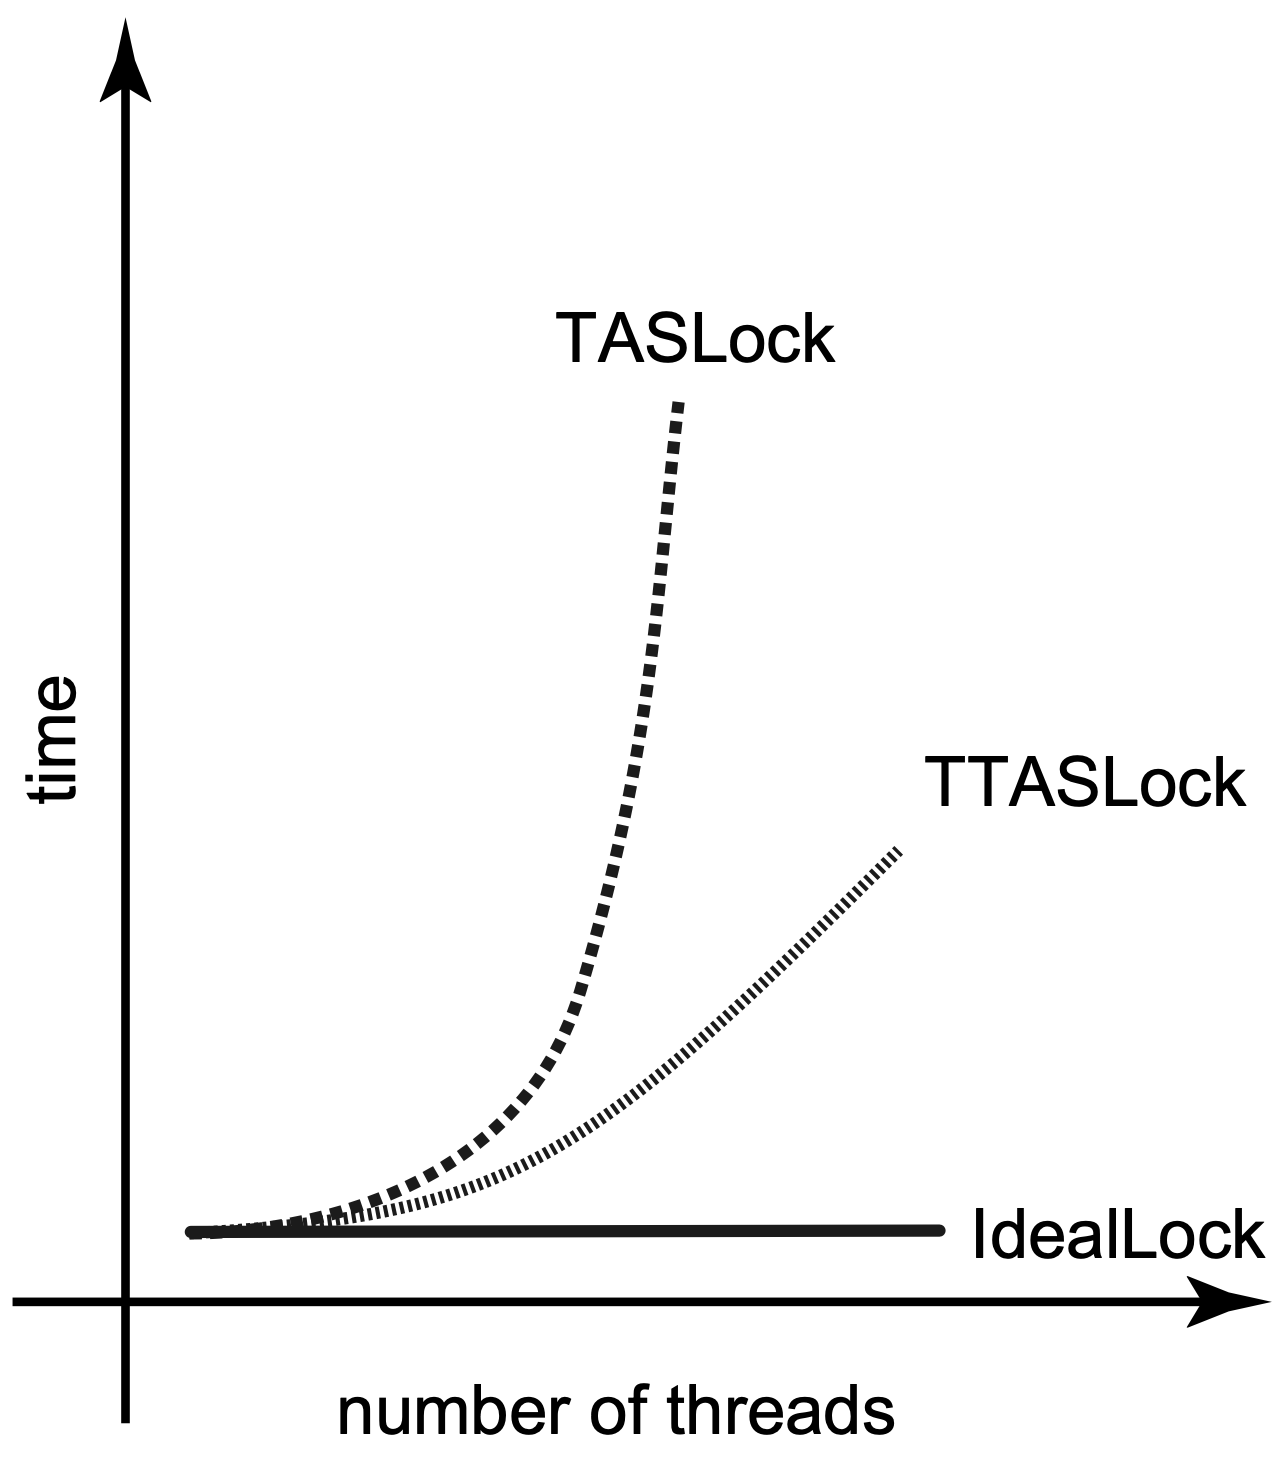
\includegraphics[width=0.4\textwidth]{fig/tas_vs_ttas.png}
\end{figure}
\end{frame}

\begin{frame}[fragile]
\frametitle{Жизненный цикл потока: yield vs sleep}
\begin{figure}[H]
\centering
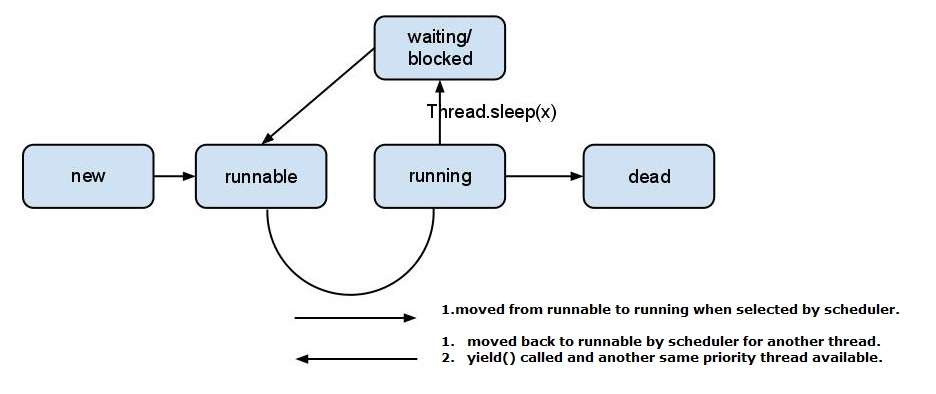
\includegraphics[width=1.0\textwidth]{fig/yield_vs_sleep.jpg}
\end{figure}
\end{frame}

\begin{frame}[fragile]
\frametitle{Как нам обустроить spin loop}
\begin{figure}[H]
\centering
\begin{minipage}{0.8\textwidth}
\begin{verbatim}
while(flag.load() == 0) {
  __asm volatile ("pause" ::: "memory");
}
\end{verbatim}
\end{minipage}
\end{figure}
\begin{figure}[H]
\centering
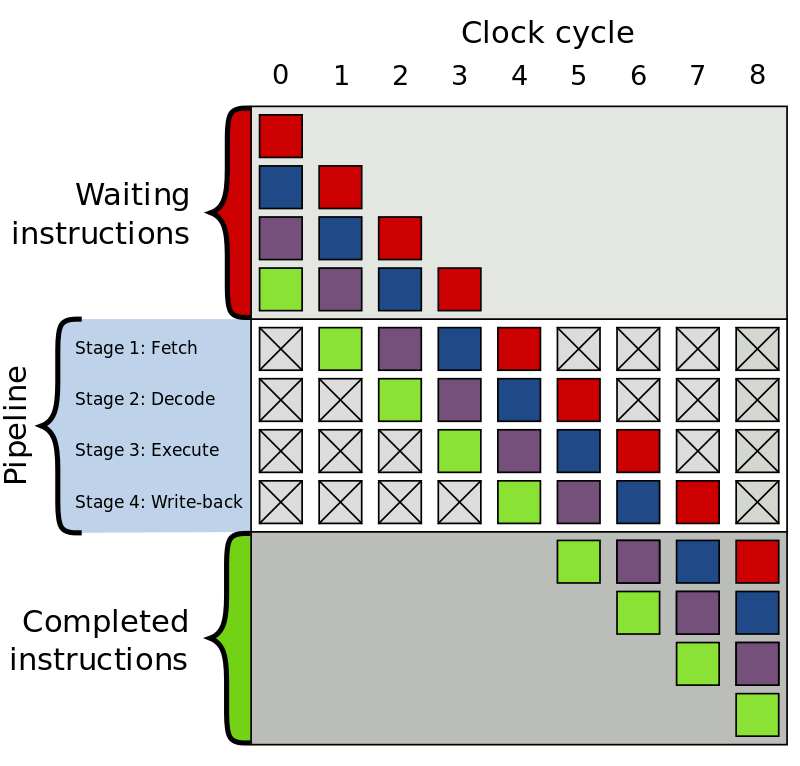
\includegraphics[width=0.4\textwidth]{fig/pipeline.png}
\end{figure}
\end{frame}

\begin{frame}[fragile]
\frametitle{Ticket lock}
\begin{figure}[H]
\centering
\begin{minipage}{0.8\textwidth}
\begin{minted}{C++}
class ticket_lock
{
    std::atomic_size_t now_serving = {0};
    std::atomic_size_t next_ticket = {0};

public:
    void lock() {
        const auto ticket = next_ticket.fetch_add(1);
        while (now_serving.load() != ticket);
    }

    void unlock() {
        const auto successor = now_serving.load() + 1;
        now_serving.store(successor);
    }
};
\end{minted}
\end{minipage}
\end{figure}
\begin{block}{Вопрос}
Как в атомарных операциях расставить \texttt{memory\_order}?
\end{block}
\end{frame}

\begin{frame}[fragile]
\frametitle{Offtop: контейнеры на Си}
\begin{figure}[H]
\centering
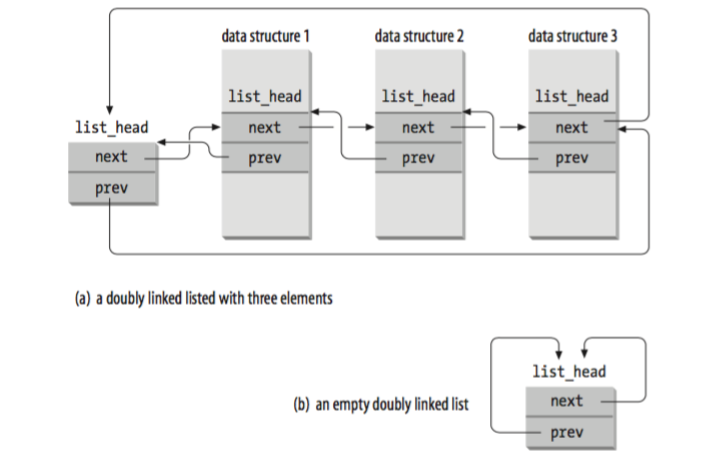
\includegraphics[width=0.7\textwidth]{fig/linux-list.png}
\end{figure}
\end{frame}

\begin{frame}[fragile]
\frametitle{Offtop: контейнеры на Си}
\begin{figure}[H]
\centering
\begin{minipage}{0.8\textwidth}
\begin{verbatim}
#include <stddef.h>
// #define offsetof(st, m) \
//     ((size_t)((char *)&((st *)0)->m - (char *)0))

#if defined(__GNUC__) || defined(__clang__)

#define container_of(ptr, type, member)                                        \
  ({                                                                           \
    const typeof(((type *)0)->member) *__mptr = (ptr);                         \
    (type *)((char *)__mptr - offsetof(type, member));                         \
  })

#elif defined(_MSC_VER)

#define container_of(ptr, type, member) (type*)((char*)ptr - offsetof(type, member))

#endif    
\end{verbatim}
\end{minipage}
\end{figure}
\end{frame}

\begin{frame}[fragile]
\frametitle{Array-based queue lock}
\begin{figure}[H]
\begin{minipage}{0.4\textwidth}
\small
\begin{minted}{C++}
class ALock {
    pthread_key_t idx_key;
    atomic<uint64_t> tail;
    atomic<uint8_t> *flag;
    size_t size;

    int get_thread_idx() {
        void *mem = pthread_getspecific(idx_key);
        return mem ? *((int*)mem) : -1;
    }

    void set_thread_idx(int val) {
        void *mem = malloc(sizeof(int));
        *((int*)mem)=val;
        pthread_setspecific(idx_key, mem);
    }
\end{minted}
\end{minipage}
\hspace{0.05\textwidth}
\begin{minipage}{0.5\textwidth}
\small
\begin{minted}{C++}
public:
    ALock(size_t cap) : tail(0), size(cap) {
        pthread_key_create(&idx_key, NULL);
        flag = new atomic<uint8_t>[cap];
        flag[0].store(1);
        for (size_t i = 1; i < cap; i++)
            flag[i].store(0);
    }

    void lock() {
        const auto idx = tail.fetch_add(1) % size;
        set_thread_idx(idx);
        while (!flag[idx].load());
    }

    void unlock() {
        const auto idx = get_thread_idx();
        flag[idx].store(0);
        flag[(idx + 1) % size].store(1);
    }
};
\end{minted}
\end{minipage}
\end{figure}
\begin{alertblock}{Замечание}
Упорядочение памяти \texttt{(memory\_order)}, обработка ошибок, деструктор класса опущены для наглядности
\end{alertblock}
\end{frame}

\begin{frame}[fragile]
\frametitle{Array-based queue lock}
\begin{figure}[H]
\centering
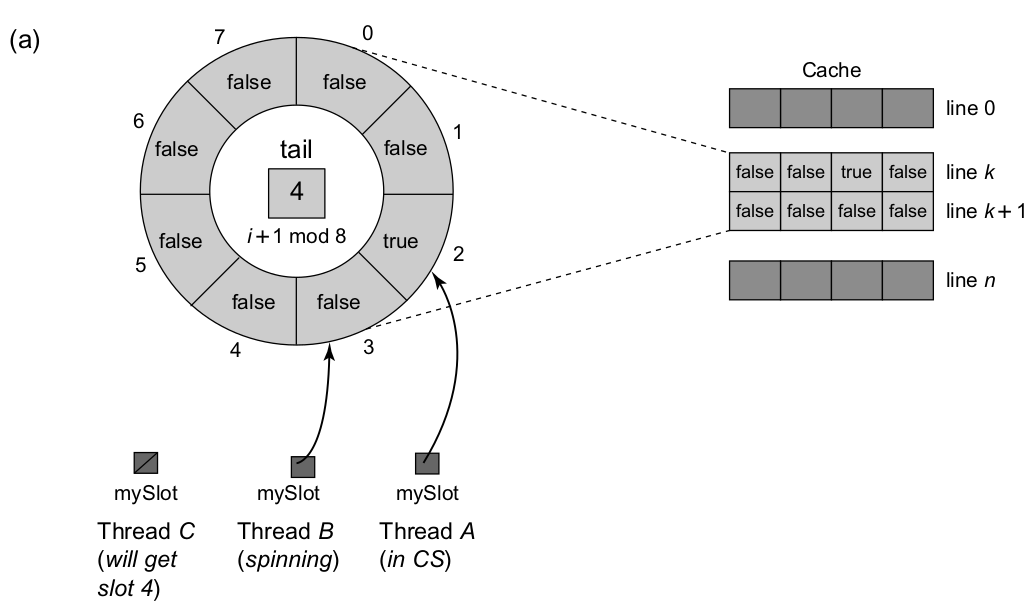
\includegraphics[width=0.45\textwidth]{fig/alock_padding-a.png}
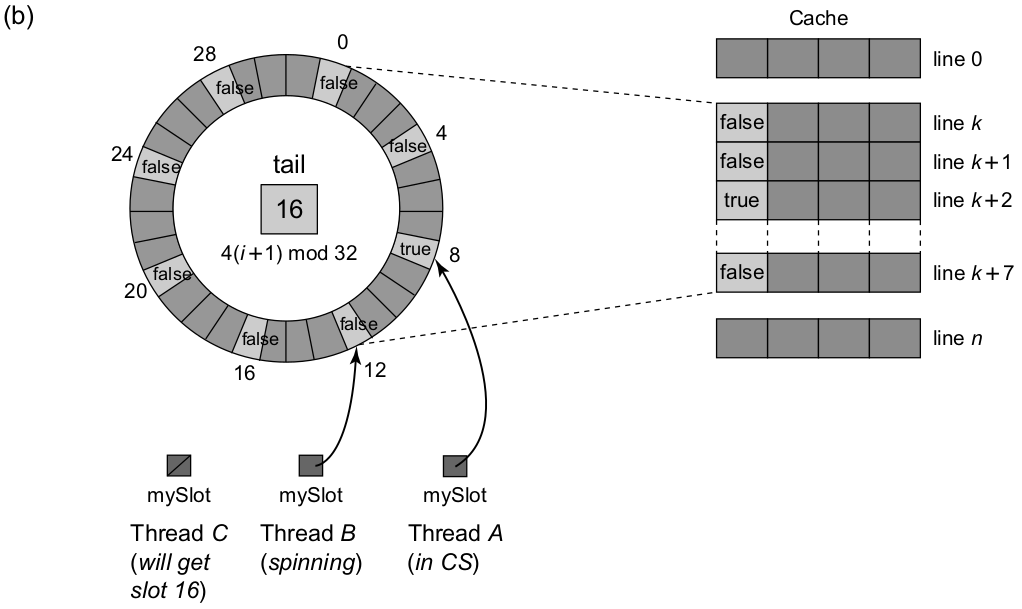
\includegraphics[width=0.45\textwidth]{fig/alock_padding-b.png}
\end{figure}
\end{frame}

\begin{frame}[fragile]
\frametitle{CLH lock}
\begin{figure}[H]
\begin{minipage}{0.8\textwidth}
\small
\begin{minted}{C}
struct clh_mutex_node {
    _Atomic char succ_must_wait;
};

typedef struct {
    clh_mutex_node_t * mynode;
    char padding[64];  // To avoid false sharing with the tail
    _Atomic (clh_mutex_node_t *) tail;
} clh_mutex_t;

static clh_mutex_node_t * clh_mutex_create_node(char islocked) {
    clh_mutex_node_t * new_node = (clh_mutex_node_t *)malloc(sizeof(clh_mutex_node_t));
    atomic_store_explicit(&new_node->succ_must_wait, islocked, memory_order_relaxed);
    return new_node;
}

void clh_mutex_init(clh_mutex_t * self) {
    // We create the first sentinel node unlocked, with islocked=0
    clh_mutex_node_t * node = clh_mutex_create_node(0);
    self->mynode = node;
    atomic_store(&self->tail, node);
}
\end{minted}
\end{minipage}
\end{figure}
\texttt{https://github.com/pramalhe/ConcurrencyFreaks/blob/master/C11/locks}
\end{frame}

\begin{frame}[fragile]
\frametitle{CLH lock}
\begin{figure}[H]
\begin{minipage}{0.8\textwidth}
\small
\begin{minted}{C}
// simplified version
void clh_mutex_lock(clh_mutex_t * self) {
    // Create the new node locked by default, setting islocked=1
    clh_mutex_node_t *mynode = clh_mutex_create_node(1);
    clh_mutex_node_t *prev = atomic_exchange(&self->tail, mynode);

    // This thread's node is now in the queue, so wait until it is its turn
    while (atomic_load(&prev->succ_must_wait));

    // This thread has acquired the lock on the mutex and it is now safe to
    // cleanup the memory of the previous node.
    free(prev);

    // Store mynode for clh_mutex_unlock() to use. We could replace
    // this with a thread-local, not sure which is faster.
    self->mynode = mynode;
}

void clh_mutex_unlock(clh_mutex_t * self) {
    if (self->mynode == NULL) {
        // ERROR: This will occur if unlock() is called without a lock()
        return;
    }
    atomic_store(&self->mynode->succ_must_wait, 0);
}
\end{minted}
\end{minipage}
\end{figure}
\end{frame}

\begin{frame}[fragile]
\frametitle{CLH lock}
\begin{figure}[H]
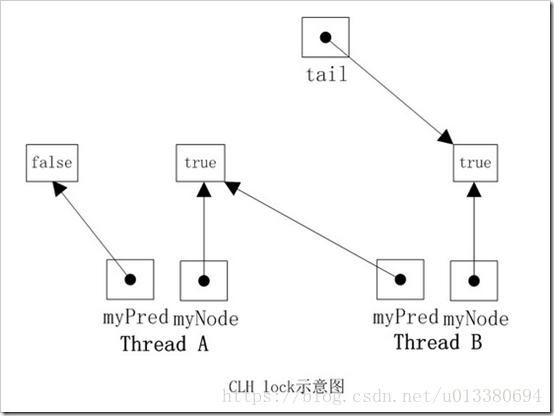
\includegraphics[width=0.5\textwidth]{fig/clh.jpeg}
\end{figure}
\end{frame}

\begin{frame}
\frametitle{Задачи}
\begin{enumerate}
\item Подумайте, как нужно поставить \texttt{memory\_order} в обращениях к атомарным переменным в примерах с семинара.
\item Можно ли обойтись без \texttt{pthreads} для организации thread-local переменных? Предложите свой вариант array-based lock.
\item \textbf{(Обязательная)} Напишите свои mutex'ы, использующие yield / exponential backoff.
    Сравните производительность TAS lock / TTAS lock / ticket lock.
    Предлагается использовать C++11 (и выше), при желании можно GNU С11 и pthreads.
\end{enumerate}

\end{frame}

\end{document}
